\chapter{O Orientador}

\begin{center}
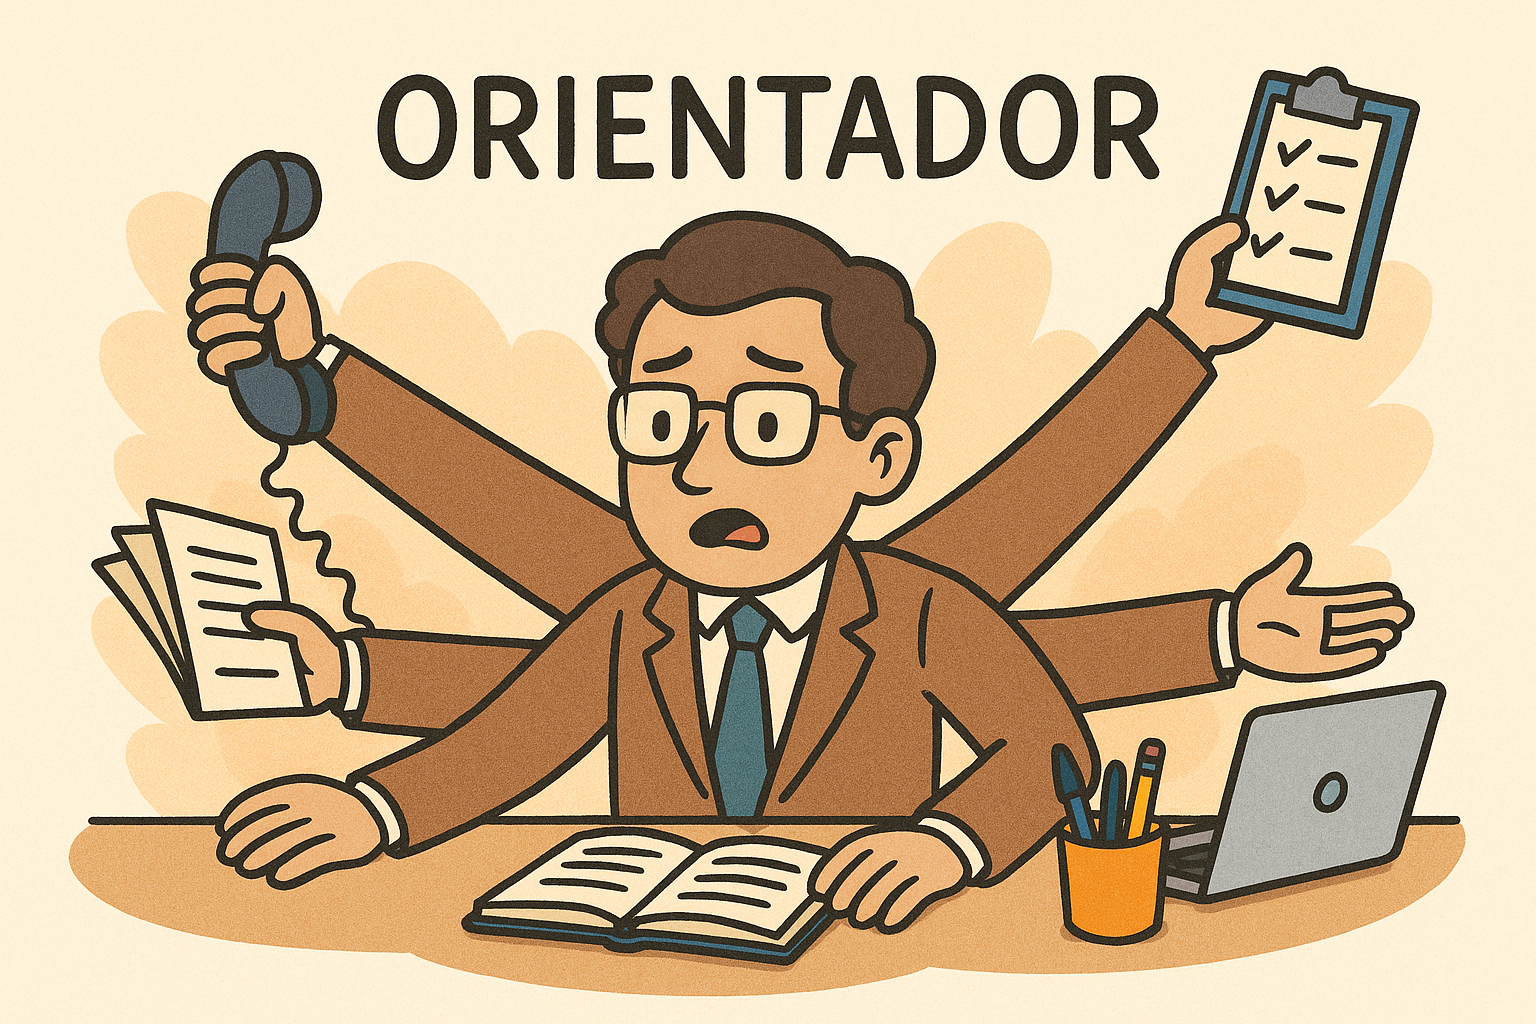
\includegraphics[width=0.5\linewidth]{Images/orientador.png}    
\end{center}
\vspace{0.5cm}

\needspace{5\baselineskip}
\section{A Expectativa do Orientador}

O orientador espera que o aluno seja ético, trabalhador e inteligente, provavelmente nessa ordem. 
Esse é o parâmetro que orientadores tentam prever no processo de seleção, tanto no inicial, quando o aluno se candidata ao curso, quanto na escolha dos orientandos\footnote{No PESC os alunos são selecionados por linha e escolhem os orientadores ao longo do curso.}

A ética é necessária tanto na pesquisa quanto no relacionamento. O orientador espera que o aluno seja honesto e transparente quanto às suas atividades e resultados.
Quando o aluno diz ``eu fiz isso'' o orientador acredita. Porém, se o aluno não tem como mostrar que fez, ou não é capaz de desenvolver raciocínios e propostas sobre o que disse ter feito, o orientador começa a duvidar e o relacionamento se degrada.

O orientador espera que o aluno trabalhe. Isso significa que ele espera um fluxo de entregas periódico, de acordo com a carga de trabalho esperada implicitamente em função do tipo de matrícula (tempo integral ou parcial). 

Finalmente, o orientador espera um grau de inteligência e conhecimento razoável. A verdade é que muitos associam o título de mestre ou doutor a uma inteligência  supostamente superior, mas, na verdade, isso não é necessário. O que é necessário é um grau de conhecimento suficiente para trazer uma contribuição relevante e dedicação. 

O orientador também espera que o aluno não perca prazos. Mais que isso, e parece estranho, ele espera que o aluno saiba quem é perante a instituição e seu status no curso e na universidade. Ele tem que saber seus códigos de matrícula, que cursos fez, que notas tirou, com que professores teve aula, quando entrou no curso, qual o órgão financiador de sua bolsa e como exige o reconhecimento da bolsa nos artigos. Se o aluno não tem essas informações a mão é como não soubesse quem é.

Uma expectativa implícita do orientador é que o aluno seja pró-ativo e não dependente. Leia o texto ``Mensagem a Garcia'' no Anexo \ref{chap:garcia}.

\needspace{5\baselineskip}
\section{A Aposta do Orientador}

Quando um orientador aceita um aluno para orientar está fazendo uma aposta. Provavelmente, quando aceitou um, deixou de aceitar outro.

Seu desempenho como aluno afeta não só a carreira do orientador, como também a carreira das pessoas que não foram selecionadas.

Isso significa que você tem uma espécie de débito não só com seu orientador, mas também com a sociedade. Você paga esse débito cumprindo sua missão: defendendo a tese. Adicionalmente, você deve realizar outras atividades acordadas tanto na aceitação quanto ao longo do curso. Elas certamente incluem publicar, mas também incluem apoiar outras atividades, participar de aulas, de laboratórios, etc. Esse trabalho inclui cumprir prazos. Novamente, quando você ultrapassa um prazo, não só prejudica seu orientador, como as outras pessoas que não vão poder ser aceitas porque você está ocupando a vaga.


\needspace{5\baselineskip}
\section{O Que Esperar do Orientador?}

No mínimo você deve exigir que o orientador seja ético e que respeite o aluno como ser humano. Práticas abusivas, apesar de acontecerem, não podem ser toleradas e devem ser denunciadas pelos canais oficiais.

Em segundo lugar, o aluno deve esperar que o orientador aloque ao seu atendimento um tempo proporcional a duas coisas:
\begin{itemize}
    \item A quantidade de alunos e outras tarefas do orientador
    \item A capacidade de resposta, ou ritmo de interação, do aluno
\end{itemize}
Isso quer dizer que um aluno que demora três meses para trazer um resultado não pode esperar que o orientador o avalie no mesmo dia. Na verdade, já conheci orientadores que tinham como norma demorar o mesmo tempo que demorou para um trabalho ser entregue para avaliar o trabalho. Há um pouco de exagero nessa regra, porém posso, como orientador, entender o porquê dessa exigência.

Assim, não se iluda, se seu orientador tem um cargo administrativo, vários projetos, muitos alunos, seu tempo será menor. Provavelmente, nesse caso, ele é um orientador experiente e seu tempo também será \textbf{melhor}, mas nem sempre isso é verdade.

O aluno também deve esperar que o orientador \textbf{oriente}, ou seja, indique caminhos para seguir e para evitar. Para isso ser bem feito, depende também da experiência do orientador, então se você escolhe um orientador muito novo, pode ter uma resposta de menor qualidade em relação a isso, mas melhor em relação a outros fatores.

Cada orientador tem um conjunto de regras, geralmente muito claras. Se você não cumpre as regras, está sujeito a consequências. Essas regras devem ser combinadas no início do trabalho.

Além desses avisos, a pergunta é: o que você espera do orientador? Que tal fazer uma lista, para ajudar no processo de escolha?

\needspace{5\baselineskip}
\section{Qual a Função do Orientador}

A função do orientador é orientar, ou seja, mostrar caminhos, estimulá-lo à pesquisa, ajudar a encontrar problemas que você possa resolver. Ele também deve ajudar com a burocracia e com problemas relacionados à universidade. 

As palavras chave são orientar e ajudar, não fazer.

Não é função do orientador resolver os problemas da sua tese. Porém, ele pode, eventualmente, dar contribuições essenciais. Não é função dele resolver suas obrigações com o curso, a não ser que ele seja explicitamente exigido.

Alguns orientadores vão ajudá-lo a resolver problemas pessoais, provavelmente apenas com conselhos, mas não é essa a sua função, isso é fruto da relação desenvolvida entre uma pessoa mais experiente e uma menos experiente. 
Porém, ele deve conhecer os problemas para entender a sua produtividade, pela necessidade de transparência no relacionamento, enquanto não é da sua obrigação resolvê-los. Se o faz, faz por vontade própria e solidariedade.

A relação orientado/orientador é muito variada, porém deve ser sempre cordial e transparente. 
Faça todos os esforços possíveis para não iniciar uma discussão pessoal com seu orientador. 

\gxatencao{O respeito é essencial}

A primeira coisa a entender é que o orientador não é orientador por ser mais inteligente que você, mas por ter mais experiência que você em uma área específica.
Muitas vezes os orientadores são mais novos que os orientados e, mesmo assim, alcançam bons resultados. 
É importante que você respeite seu orientador.

\needspace{5\baselineskip}
\section{Dificuldades comuns com os orientadores}


Normalmente, seu orientador o tratará com respeito, porém os seguintes problemas podem aparecer:

\begin{outline}
\1	O orientador não tem tempo para você
\1	O orientador não leu o que você escreveu
\1	O orientador não entende o que você faz
\end{outline}

\subsection{O Orientador sem tempo}


É comum um orientador ter pouco tempo disponível. Ele tem que dar aulas, participar de reuniões, orientar outros alunos e realizar atividades como pesquisa e consultoria. Você deve se adaptar ao tempo disponível de seu orientador. 

\gxatencao{O orientado deve se adaptar aos horários do orientador, não o contrário.}

Algumas desculpas são inaceitáveis pelo orientador e entre elas está que ``você não pode sair de seu trabalho nessa hora''. Afinal, você está ou não fazendo uma tese? É possível, porém, que seu orientador concorde em o orientar na casa dele, após o expediente, e, em casos excepcionais, no fim de semana. Não é o meu caso e acredito que, tirando condições excepcionais, não deveria ser o caso de nenhum orientador.

Caso seu orientador tenha problemas graves na agenda, tente marcar um almoço com ele. Outra opção é conseguir um coorientador, outro professor da mesma área ou um aluno de doutorado, caso você seja aluno de mestrado. Muitos orientadores gostam de trabalhar no regime de dupla orientação.


\subsection{O orientador que não leu o que você escreveu}


Se o orientador não leu o que você escreveu é porque não teve tempo ou esqueceu. Se ao encontrar seu orientador ele não tiver lido o que você escreveu, faça um resumo mostrando o texto para ele. Raramente o orientador é ``preguiçoso'' ou ``desatento'', mas frequentemente é sobrecarregado. 


\gxatencao{Sempre leve uma cópia do trabalho que você está fazendo para as reuniões. }


Aparecer em uma reunião sem isso é demonstrar desinteresse pela reunião, falta de preparação ou, pior, que você não fez nada.

Muitos orientadores leem um texto por alto e ficam com uma ideia muito clara do que foi feito. Principalmente nos casos de revisão bibliográfica e resultados demonstrados em gráficos, o orientador pode, em 10 ou 15 minutos, ter uma ideia clara do seu trabalho e contribuir para o seu desenvolvimento. 


É importante entender que o esforço do orientador é muito relacionado ao esforço do aluno. Alguns alunos parecem frustrados porque o orientador, na segunda ou terceira vez que eles aparecem com o trabalho no mesmo estágio, não está disposto a conversar por muito tempo ou dar ideias. Essa reação não é nada surpreendente, se você não faz o seu trabalho, o orientador não tem como fazer o dele.


\gxatencao{Um processo de orientação se baseia na evolução do trabalho do orientado.}


\subsection{O orientador que não entende o que você faz}

Das três situações que citei, essa é a mais difícil de resolver.

Não é raro que um aluno desenvolva um assunto de tese que foge dos conhecimentos do orientador. Nesse caso, muitos orientadores coíbem o desenvolvimento da tese, enquanto outros buscam soluções de compromisso. Outros podem entender como uma oportunidade de abordar novas áreas. Na verdade, dependendo do assunto, a disposição do orientador pode mudar.

Uma coorientação pode, novamente, ser uma boa solução. Uma revisão bibliográfica também pode dar ao orientador as ferramentas necessárias para auxiliar no seu trabalho. Em geral, um orientador fica feliz se seu aluno sabe mais que ele sobre um assunto.


\needspace{5\baselineskip}
\section{Mais sobre os orientadores}


Os orientadores também passam por ciclos de alta imaginação e excessiva realidade. Muitas conversas serão ``viagens'' e outras serão ``convocações para pôr o pé no chão''. De certa forma, essa é a tarefa do orientador. Se você estiver viajando pouco, ele vai tentar desenvolver os limites da sua imaginação; se você estiver passeando no espaço sideral, ele vai tentar trazê-lo de volta para a realidade.


As conversas com o orientador devem ser plenamente documentadas, pelo aluno, mesmo que o orientador faça isso. Se os dois estiverem documentando a conversação, compare as notas no final. 


\gxatencao{O aluno deve sair de cada conversa com uma lista de itens a fazer}


Se seu orientador não criar essa lista, pergunte diretamente quais devem ser seus próximos passos ou sugira você mesmo uma lista de ações. 


Entre duas sessões de orientação, seu orientador certamente mudará de ideia. 


\gxatencao{Nunca jogue fora um trabalho anteriormente descartado}


Caso um assunto previamente descartado como ``ruim'' seja considerado ``bom'' em uma reunião posterior, verifique em suas anotações o motivo da decisão anterior e discuta-os com o orientador. Porém, tente não questionar a mudança de opinião, pois isso só vai levar a um sermão sobre a necessidade de se ter uma mente aberta e pronta para mudanças. Revise os defeitos e qualidades da opção sendo estudada e tome uma nova decisão.


Existem muitos tipos de orientadores: o viajante, o amigão, o carrasco, o executivo, o objetivo etc. Todos esses têm suas vantagens e desvantagens, cabe a você descobrir quais os defeitos do seu orientador e evitar que eles tenham má influência na sua tese. Se seu orientador tem muitas ideias, você deve ser objetivo, se seu orientador é relapso com prazos, você deve cumprir todos. Orientadores são seres humanos e têm defeitos, muitas vezes graves. 


Só você pode evitar que esses defeitos influenciem na sua tese. Quanto aos seus defeitos, fique certo de que o orientador irá apontá-los no decorrer do relacionamento, algumas vezes até de maneira um tanto rude.

\needspace{5\baselineskip}
\section{Confiança no orientador}


O maior desejo do orientador é que o aluno termine a tese. É quase inconcebível imaginar que um orientador não deseje que o aluno complete o mais rápido possível e da melhor forma, o seu trabalho. 

Por que falo isso com tanta certeza? Porque os professores são avaliados, parcialmente, pela capacidade de fazer seus alunos defenderem suas teses e publicarem artigos sobre elas.

Alguns alunos, porém, imaginam que o professor está contra eles. Acham que estão pedindo trabalhos impossíveis, apenas para o benefício próprio, ou pior, para atrapalhá-los.

A verdade é que cada orientador determina um nível de qualidade aceitável para o trabalho do aluno. Esse nível é compatível com as características do aluno. 
Assim, um aluno capaz de fazer ótimos programas de computador, mas péssimo em teoria, é estimulado, e cobrado, a explorar suas qualidades ao máximo e a lutar, na medida do possível e do aceitável, contra suas dificuldades.

O orientador trabalha \textbf{sempre a favor do aluno}, dentro de algumas restrições pessoais e institucionais. 
Essas restrições envolvem a área de pesquisa, a qualidade do resultado, a dedicação ao trabalho e muitos outros fatores. 
Poucas vezes um orientador reprova ou abandona um aluno.
 Ele sempre tenta ao máximo encontrar um caminho de sucesso. 
 Essa é a tarefa principal do orientador.

Uma restrição importante que todo aluno deve estar atento é que a carreira acadêmica do orientador é fortemente, se não unicamente, influenciada pela quantidade e qualidade de suas publicações. 
O orientador é um professor que tem que arcar com muitas responsabilidades: aulas, administração da faculdade, orientação e escrever artigos. 
Assim, os orientadores normalmente esperam que o orientado os auxiliem na tarefa de escrever artigos. 

Os alunos que desejam seguir carreira acadêmica devem ficar especialmente preocupados em publicar, afinal, eles também serão julgados por sua capacidade de produção de artigos.

\gxatencao{Assim, o aluno deve estabelecer uma relação de confiança e colaboração com seu orientador.}

\needspace{5\baselineskip}
\section{A Escolha}


A escolha do orientador é um processo bastante complicado. Alguns alunos não têm essa opção, pois são selecionados desde o início para serem orientados por um professor. 


% Você pode analisar um orientador de acordo com as várias facetas, como:
% \begin{enumerate}
% 	\item 	Compatibilidade pessoal;
% 	\item 	Assuntos comuns;
%     \item Histórico de trabalho conjunto;
% 	\item 	Qualidade como; orientador;
% 	\item 	Qualidade como professor;
% 	\item 	Qualidade como pesquisador;
%     \item Qualidade como líder de equipe;
%     \item Importância na área, e, sem esgotar os motivos,
% 	\item 	Opinião pessoal.
% \end{enumerate}

A escolha do orientador é uma das decisões mais importantes da vida acadêmica de um estudante de pós-graduação. Mais do que um supervisor técnico, o orientador será, por um período considerável, um parceiro de trabalho intelectual, uma referência profissional e, muitas vezes, uma figura central na formação científica do aluno. Por isso, é fundamental analisar essa escolha a partir de múltiplas facetas:

\begin{itemize}
\item \textbf{Compatibilidade pessoal:} A relação entre orientador e orientando é, em muitos aspectos, uma parceria. Diferenças de temperamento, estilo de comunicação, expectativas e ritmo de trabalho podem gerar atritos ou frustrações. Um bom relacionamento interpessoal favorece a confiança, o diálogo aberto e a resolução construtiva de conflitos.

\item \textbf{Assuntos comuns:} É importante que o orientador tenha interesse ou experiência na temática que o aluno deseja desenvolver. Ainda que o projeto possa ser reformulado, trabalhar em uma área próxima dos interesses do orientador aumenta a qualidade da orientação e facilita o acesso a bibliografia, eventos e redes de pesquisa relevantes.

\item \textbf{Histórico de trabalho conjunto:} Se o aluno já teve experiências anteriores com o possível orientador — em disciplinas, iniciação científica, monitorias ou projetos — isso oferece pistas concretas sobre como será a convivência e a orientação. Um histórico positivo tende a reduzir incertezas.

\item \textbf{Qualidade como orientador:} Nem todo bom pesquisador é, necessariamente, um bom orientador. Essa qualidade diz respeito à capacidade de guiar o aluno em sua trajetória acadêmica com equilíbrio entre autonomia e suporte, respeitando os prazos e o estilo de trabalho do orientando. Um bom orientador também estimula o pensamento crítico e oferece retornos construtivos e frequentes.

\item \textbf{Qualidade como professor:} Professores que são didáticos, acessíveis e organizados em suas disciplinas frequentemente também trazem essas qualidades para a orientação. Um docente comprometido com a formação discente tende a cultivar uma postura pedagógica também fora da sala de aula.

\item \textbf{Qualidade como pesquisador:} Um orientador com produção científica relevante pode abrir portas para colaborações, publicações e visibilidade acadêmica. Além disso, tende a estar atualizado com os debates da área e pode contribuir com sugestões mais consistentes para o desenvolvimento do projeto.

\item \textbf{Qualidade como líder de equipe:} Muitos orientadores coordenam grupos de pesquisa. Saber liderar um grupo, distribuir tarefas de forma justa, conseguir financiamentos, manter um ambiente de respeito e estimular a colaboração são características que impactam diretamente a experiência do aluno, especialmente em trabalhos coletivos ou interdisciplinares.

\item \textbf{Importância na área:} Um orientador reconhecido nacional ou internacionalmente pode trazer benefícios indiretos, como recomendações mais influentes, oportunidades de intercâmbio, maior facilidade de aprovação em bolsas e financiamentos, e visibilidade para o trabalho do aluno. No entanto, esse fator não deve se sobrepor à qualidade da relação pessoal e à disponibilidade efetiva do orientador.

\item \textbf{Opinião pessoal:} Por fim, é legítimo considerar a impressão pessoal do aluno. Intuições e percepções subjetivas, quando baseadas em observações concretas, podem sinalizar afinidades ou riscos que não são capturados por critérios objetivos. O aluno deve se sentir confortável e confiante para desenvolver seu trabalho com aquele orientador.

\end{itemize}


Existem muitas maneiras de iniciar essa seleção. Normalmente você deve ter como opção os professores que admira ou  com os quais já fez alguma cadeira ou trabalho. 
Seus colegas mais antigos também são capazes de dar informações sobre os professores disponíveis.
Além disso, muitas vezes outros professores podem recomendar um colega, de acordo com seus objetivos como aluno.


Um conselho importante é não se assustar muito com orientadores com fama de durões. 
Um orientador durão pode ser um ótimo orientador e manter você nos ``trilhos certos''. Cuidado, porém, com os que têm fama de mal-educados e abusivos.

\needspace{5\baselineskip}
\section{Problemas com o orientador}

Aconteceu! Você discutiu com seu orientador de forma irreconciliável ou se acha prejudicado fortemente, ou acha que não pode continuar trabalhando com ele. 
O que fazer?

Vamos tratar primeiro de problemas onde não há uma questão legal, isso é, problemas de relacionamento que não incluem atos como assédio sexual, racismo, etc.

Primeiro, respire. 
É importante parar para pensar, pois existe um registro histórico que é desfavorável a você: seu orientador já orientou diversos alunos e trabalhos; você não fez nenhuma tese.

É fato que todo relacionamento de longo prazo está sujeito a turbulências. \textbf{Namoros e casamentos acabam, por que uma orientação não pode acabar?} 
O problema é que, nesse caso, se não houve uma quebra da ética, regulamento ou lei, ou seja, é apenas um desacordo agravado de alguma forma, normalmente apenas um lado é prejudicado: o aluno.

Para resolver o problema, temos que pensar em um escalonamento de soluções. 

Por incrível que pareça, no caso de desacordos, a primeira pessoa que pode ajudá-lo é o próprio orientador. 
Se ainda for possível, tente marcar outra reunião e, de forma educada, dizer que não consegue mais trabalhar nas condições atuais. 
Lembre-se que, sendo a parte mais frágil, acusar pouco vai servir a você. 
Seu orientador então pode se propor a buscar um novo orientador ou um coorientador, ou pedir que você o faça. 
Essa solução é a mais fácil. Talvez não seja suficiente.

A seguir, caso isso não funcione, ou o caso seja tão  grave que não pode ser tratado com o próprio orientador ou orientadora, você deve caminhar pelas instâncias da instituição.. 
Certamente, seu programa de pós-graduação tem um coordenador, mas pode haver outros cargos relevantes, como o coordenador acadêmico, ou um responsável por relações com os alunos, e possivelmente a instituição tem uma ouvidoria que pode te ajudar. 
Além disso, em muitos lugares, os alunos são bem organizados e possuem um grêmio acadêmico ou associação de alunos que pode ajudar. 

Ainda tratando de casos ``normais'' de desacordo, recomendo não pular etapas. Você pode ir na instância mais alta da universidade em busca de seus direitos, mas isso deve ser feito passo a passo.

No caso de questões que constituem crime, acho importante \textbf{buscar o apoio de um advogado} e, se for recomendado por ele, fazer a denúncia formal. 

\CoppeWay{Qual o caminho no PESC e na Coppe?}
{
No Programa de Engenharia de Sistemas e Computação da  Coppe existe um chefe de linha, a coordenação acadêmica e o coordenador. 
No nível da Instituição, a Coppe, ainda existe o Coordenador Acadêmico e o Conselho de Pós-Graduação e Pesquisa(CPGP). 

Historicamente, já vi serem criados processos administrativos formais contra professores.
}

Não confunda, porém, exigência com abuso. Se o orientador diz que seu trabalho está ruim, a minha experiência diz que é muito provável que esteja mesmo. 
Porém, já vi poucos casos onde o orientador não entendeu o trabalho do aluno, e sua dificuldade, e por isso não o aceitava. 
Quando isso acontece, há a possibilidade de explicar não só o trabalho, mas qual a relevância dele dentro da literatura atual. Para isso, é importante ter uma boa revisão da literatura.




